\documentclass[
    10pt,
    a4paper,
    % listof = totoc
]{scrartcl}
\usepackage{ucs}
\usepackage[utf8x]{inputenc}
\usepackage[english,ngerman]{babel}
\selectlanguage{ngerman}
\usepackage[T1]{fontenc}

% Math stuff
\usepackage{amsmath}
\usepackage{amsfonts}
\usepackage{amssymb}

% Farben
\usepackage[usenames,x11names,dvipsnames,rgb]{xcolor}
\definecolor{grey}{rgb}{0.4,0.4,0.4}
\definecolor{lightgrey}{rgb}{0.8,0.8,0.8}
\definecolor{ultralightgrey}{rgb}{0.96,0.96,0.96}

% Grafix
\usepackage{graphicx}

% Schriften
\usepackage{mathpazo,avant,courier}

% TikZ (dot2tex etc.)
% \usepackage{tikz}
% \usetikzlibrary{decorations, arrows, shapes}

% Farben in Tabellen
\usepackage{colortbl}

% Lange Tabellen
\usepackage{longtable}

% Gewrappte boxen (können innerhalb f{rame}box's verwendet werden)
\usepackage{minibox}

% FloatBarrier stellt z.B. sicher, dass das Literaturverzeichnis am Ende des
% Dokuments erscheint.
\usepackage{placeins}

% Hyperref
\usepackage{hyperref}
% Hypersetup
\hypersetup{
    pdftitle = {ES-HH - Software Design ras-weather},
    pdfauthor = {David Daniel},
    pdfsubject = {Software Design ras-weather},
    pdfkeywords = {Software Design} {ES-HH},
    % hidelinks
    colorlinks = true,
    linkcolor = blue,
    % urlcolor = black
    urlcolor = Blue,
    citecolor = grey
}
\urlstyle{same}

% Apa cite style
\usepackage{apacite}

% Glossar (load _after_ ! hyperref)
% \usepackage[toc]{glossaries}
% \makeglossaries
% \newglossaryentry{RTTI}
% {
    % name = {RTTI},
    % description = {"``Run time type information"'' liefert Informationen über
    % benutzerdefinierte Typen zur Laufzeit}
% }

% Listings
% @see http://tex.stackexchange.com/questions/51867/koma-warning-about-toc
% \usepackage{scrhack}
% \usepackage{listings}
% \lstset{
    % breakatwhitespace=true,
    % columns=fullflexible,
    % keepspaces=true,
    % breaklines=true,
    % tabsize=4, 
    % showstringspaces=false,
    % extendedchars=true,
    % basicstyle=\footnotesize\ttfamily,
    % numbers=left,
    % numberstyle=\scriptsize,
    % firstnumber=1
% }
% \lstdefinestyle{custom}{
    % belowcaptionskip=1\baselineskip,
    % captionpos = b,
    % breaklines=true,
    % frame=l,
    % xleftmargin=\parindent,
    % showstringspaces=false,
    % keywordstyle=\bfseries\color{green!40!black},
    % commentstyle=\itshape\color{purple!40!black},
    % identifierstyle=\color{blue},
    % stringstyle=\color{orange},
% }

\title{ES-HH - Software Design}
% \subtitle{}
\author{Andreas Hasler \\{\small andreas.hasler@students.ffhs.ch}
\and David Daniel\\{\small david.daniel@students.ffhs.ch}}
\date{\today}

\begin{document}
\maketitle
\pagenumbering{Alph}% Use uppercase alphabetic page numbers (and reset to A)

\begin{abstract}
    Dieses Dokument erläutert die Architekturüberlegungen zum Software Design für
    ras-weather. Die hier diskutierte Architektur bezieht sich auf die Software, welche
    auf dem Raspberry Pi betrieben wird. Externe Software wie die Web-Applikation oder die
    Smartphone Applikation werden in diesem Dokument nicht beschrieben.
\end{abstract}

\clearpage
\pagenumbering{Roman}% Use uppercase roman page numbers (and reset to I)
\tableofcontents

\section{Analyse}
\pagenumbering{arabic}% Use numeric page numbers (and reset to 1)

Auf dem Raspberry Pi wird eine Software betrieben, welche zusammenfassend
\cite{project-doc} die folgenden Funktionalitäten bietet:
\begin{itemize}
    \item Nach Einschalten des Gerätes werden die aktuellen Messwerte wie Temperatur und
        Luftdruck auf dem Display angezeigt.
    \item Die Messwerte werden in periodischen Abständen in der Datenbank gespeichert.
    \item Auf Knopfdruck kann der Anwender die IP Adresse anzeigen lassen, resp. es ist
        möglich, mittels Knopfdruck die Anzeige zwischen den Messwerten und der IP Adresse
        zu wechseln.
\end{itemize}

Somit handelt es sich um die folgenden Komponenten, welche miteinander kommunizieren:

\begin{itemize}
    \item LCD
    \item Sensoren
    \item Datenbank
    \item Schalter
\end{itemize}

Da die Anwendung nach dem Einschalten des Gerätes nicht mehr gestoppt wird, bis das Gerät
ausgeschaltet wird, handelt es sich um einen Prozess, welcher im Hintergrund läuft. Dieser
Prozess ermittelt die Messwerte von den Sensoren, speichert diese in der Datenbank und
stellt die Werte auf dem LCD dar. Somit benötigt der Prozess während der gesamten Laufzeit
Zugriff auf die genannten Komponenten.

\subsection{Sensoren}
Die Sensoren werden periodisch von der Anwendung abgefragt. Zudem soll das Display die
Anzeige aktualisieren, sobald sich ein Wert ändert. Es wird daher eine Möglichkeit
benötigt, auf Ereignisse bezüglich der gemessenen Werte eines Sensors reagieren zu können.
Ein Sensor benötigt daher eine Beobachter Schnittstelle und die Möglichkeit, die aktuellen
Messwerte zu liefern.

\subsection{Datenbank}
Eine Sammlung von Messwerten wird schliesslich in der Datenbank abgelegt, zu welcher
folglich ein entsprechendes Schema folgende Felder umfasst (ohne Primärschlüssel):
\begin{itemize}
    \item Temperatur
    \item Luftdruck
    \item Lichtstärke
    \item Feuchtigkeit
    \item Datum, Uhrzeit~\footnote{Datum und Uhrzeit der Erstellung der Messwerte}
\end{itemize}

Das Auslesen der Messwerte aus der Datenbank wird durch eine andere Anwendung durchgeführt
(Web-Anwendung), daher muss die Abstraktion, welche hier eingesetzt wird, dies vorerst
nicht unterstützen.

\subsection{LCD}
Das LCD wird zur Darstellung von verschiedenen Werten verwendet, darin werden sowohl
Messwerte mit unterschiedlichen Einheiten (Grad, Pascal oder hPa, Prozent etc.) sowie die
IP Adresse und evtl. auch die Zeit dargestellt. Aufgrund des beschränkten Platzes auf dem
Display wäre es schwierig, dem Anwender des Displays freizustellen, wie der anzuzeigende
Inhalt auf dem Display dargestellt werden soll. Das Gerät muss lediglich die gewünschten
Werte auf dem Display darstellen, es reicht daher, wenn die Abstraktion des Displays dies
entsprechend ermöglicht. Somit muss das Display eine Möglichkeit bieten, einen Text wie
die IP Adresse, eine Temperatur etc. oder alle aktuellen Messwerte zugleich anzuzeigen.

Durch die Notwendigkeit, dass das Display die Anzeige aktualisiert, was das Beobachten der
Sensoren bedingt, bietet es sich an, einen klassischen Model-View Ansatz zu verfolgen. Die
Sensoren bilden so das Model, währenddem das Display als View auf Änderungen am Model
lauscht.

\subsection{Schalter}
Der oder die Schalter fungieren als Botschafter, welche die Anwendung benachrichtigen,
sobald ein Schalter gedrückt wurde. Hierzu bietet sich daher ebenfalls ein klassisches
Beobachter Modell an.

\section{Synthese}

\subsection{Ablauf}

Die Anwendung ermittelt in periodischen Zeitabständen die aktuellen Messwerte und
speichert diese in der Datenbank. Auf Anfrage über einen Schalter wechselt die Anwendung
die Anzeige und stellt den gewünschten Wert dar. Das periodische Speichern der Werte
beeinflusst jedoch nicht die Anzeige, für die Anzweige werden stets aktuelle Werte
ermittelt. Sobald die Anzeige wechselt, wird der entsprechende Wert ermittelt und
angezeigt. Anschliessend werden Änderungen des aktuell dargestellten Wertes registriert
und bei jeder Änderung wird die Anzeige aktualisiert. Der Ablauf ist im Sequenz Diagramm
in Abbildung \ref{fig:sequence-diagram} ersichtlich.

\begin{figure}[ht]
    \centering
    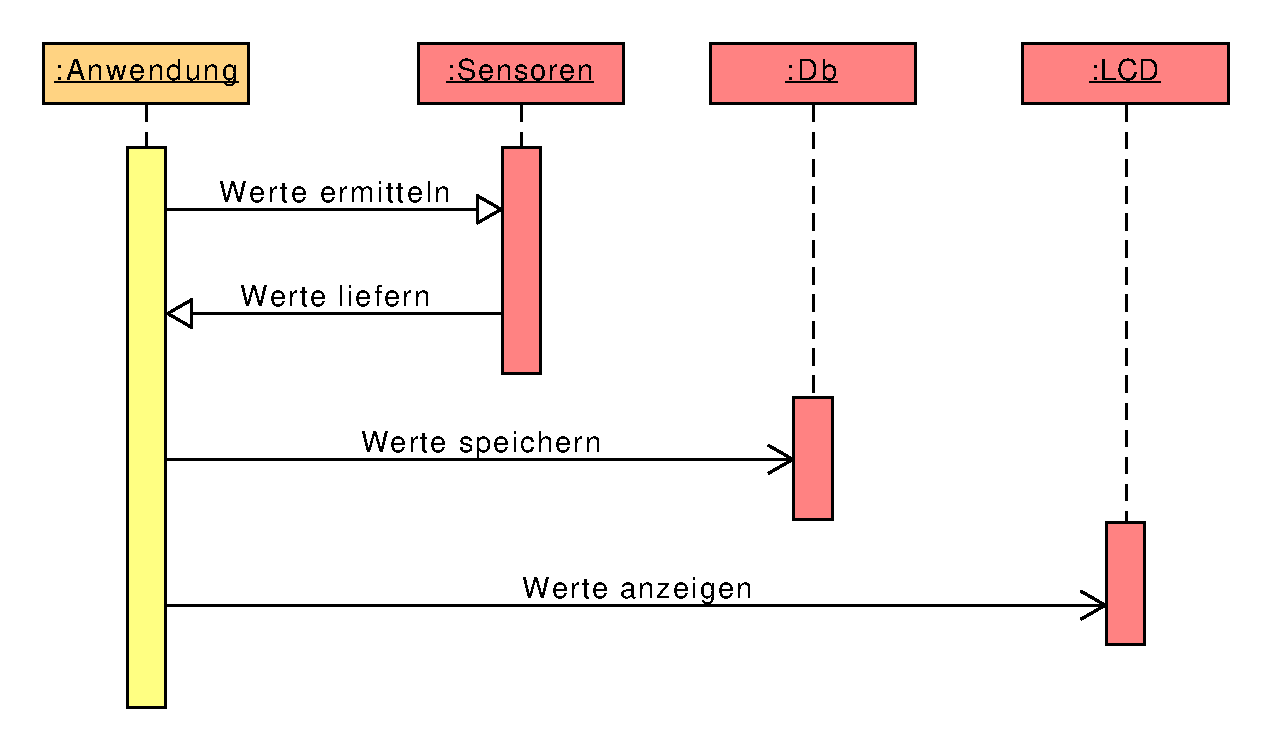
\includegraphics[width=\textwidth]{sequence-diagram}
    \caption{Sequenz Diagramm}
    \label{fig:sequence-diagram}
\end{figure}

\subsection{Abstraktionen}
Somit ergeben sich die folgenden Klassen resp. Abstraktionen mit ihren Eigenschaften und
Methoden:

\begin{itemize}
    \item Sensoren
        \begin{itemize}
            \item Alle Sensoren bieten die Möglichkeit, den aktuellen Messwert zu
                ermitteln und einen Beobachter zu benachrichtigen, sobald der aktuelle Wert
                signifikant~\footnote{Mit signifikant ist gemeint, dass sich der Wert mind. soweit
                geändert hat, als dass die Änderung auf dem Display erkennbar ist.}.
                Folgende Sensoren werden benötigt:
                \begin{itemize}
                    \item Temperatur-Sensor
                    \item Feuchtigkeits-Sensor
                    \item Luftdruck-Sensor
                    \item Licht-Sensor
                \end{itemize}
        \end{itemize}
    \item Datenbank
        \begin{itemize}
            \item Die Datenbank muss eine Menge von Messwerten (Temperatur, Luftdruck
                etc.) mit dem aktuellen Zeitstempel speichern.
        \end{itemize}
    \item LCD
        \begin{itemize}
            \item Das Display muss die folgenden Elemente darstellen können:
                \begin{itemize}
                    \item Die aktuellen Messwerte
                    \item Die IP Adresse des Gerätes
                    \item Eine Fehlermeldung
                \end{itemize}
        \end{itemize}
    \item Schalter
        \begin{itemize}
            \item Der Schalter bietet die Möglichkeit, einen Beobachter zu registrieren,
                welcher nach dem Betätigen des Schalters benachrichtigt wird.
        \end{itemize}
\end{itemize}

\subsection{Struktur}
Die Anwendung befindet sich im laufenden Zustand, sobald das Gerät gestartet wird. Sie
wird bis zum Herunterfahren des Gerätes nicht mehr gestoppt. Es handelt sich also um einen
Dämon, welcher über geeignete Massnahmen dazu bewegt werden muss, die Werte auszulesen,
diese zu speichern und auf dem Display anzuzeigen. Zudem kann der Anwender die Anzeige auf
dem Display wechseln, resp. er kann den anzuzeigenden Wert wählen oder die IP Adresse
anzeigen lassen.

Das Auslesen und Abspeichern der Werte läuft vollkommen automatisch im Hintergrund ab,
diesen Vorgang kann der Benutzer nicht beeinflussen. Daher kann dies in einem eigenen
Thread abgearbeitet werden, welcher während der gesamten Laufzeit des Dämons aktiv ist.
Für den Wechsel der Anzeige muss der Dämon resp. die zugehörige Einheit auf Tastendruck
und auf Änderungen des angezeigten Wertes reagieren.

Zusammenfassend ergibt sich die Klassenstruktur wie sie in Abbildung
\ref{fig:class-diagram} dargestellt ist.

\begin{figure}[ht]
    \centering
    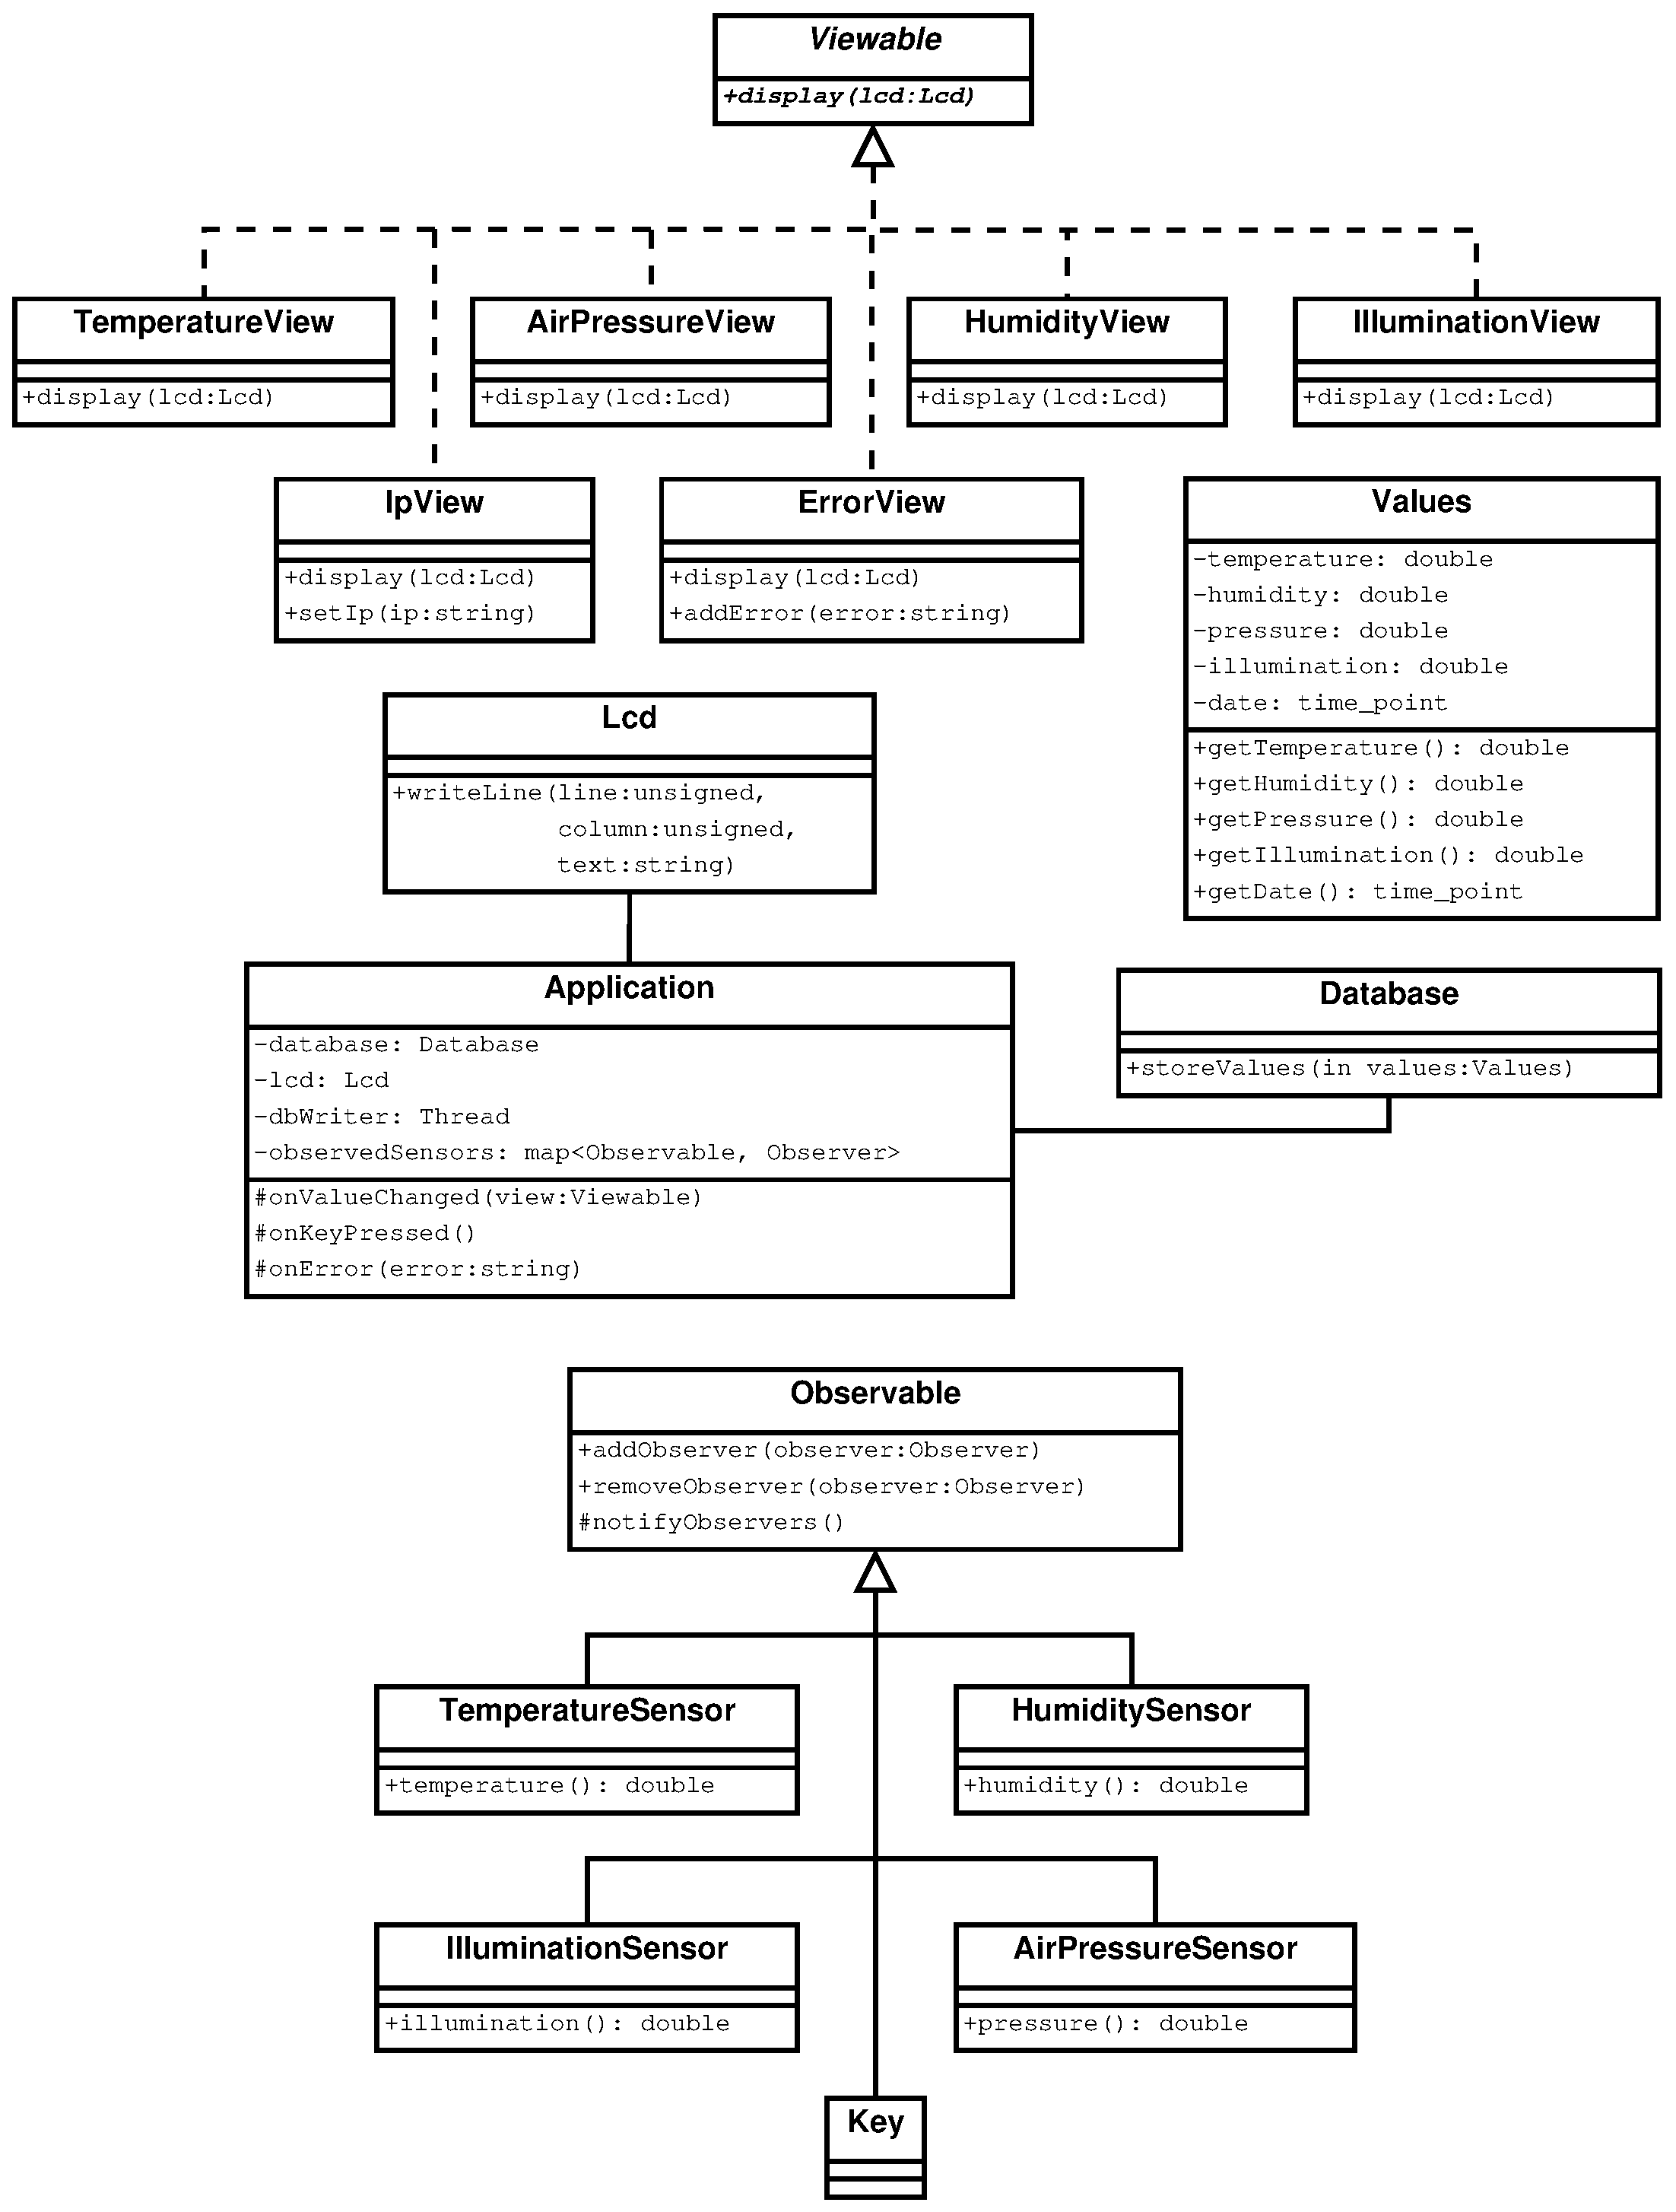
\includegraphics[width=\textwidth]{class-diagram.eps}
    \caption{Klassen Diagramm}
    \label{fig:class-diagram}
\end{figure}

\section{Verifikation}
Um den korrekten Betrieb der Software sicher zu stellen, werden in erster Linie die
möglichen Fehlerquellen ermittelt. Jede Komponente der Software und der Hardware kann
Fehler produzieren oder auslösen. Externe Fehlerquellen wie ein Ausfall der Stromzufuhr
werden ignoriert, solche Fehler können nicht adressiert werden. Ein Ausfall des LCD oder
ein festsitzender Schalter können ebenfalls nicht adressiert werden. Es bleiben daher
die folgenden möglichen Fehler, welche behandelt werden müssen:

\begin{itemize}
    \item Sensoren
        \begin{itemize}
            \item Liefern von falschen Werten (durch falsche Berechnung)
            \item Ausfall der physischen Sensoren
        \end{itemize}
    \item Datenbank
        \begin{itemize}
            \item Korrupte Daten
            \item Kein Speicherplatz mehr verfügbar
        \end{itemize}
\end{itemize}

Das Liefern von falschen Werten kann mittels Testing vermieden werden, resp. es kann
mittels manuellem Testing verifiziert werden, dass die berechneten Werte in einem
Toleranzbereich liegen. Der Ausfall der Sensoren sollte von der Anwendung erkannt werden,
es sollten keine falschen Werte angezeigt oder gespeichert werden, stattdessen sollen im
Falle von ausgefallenen Sensoren die entsprechenden Werte ignoriert werden. Die Temperatur
beträgt in diesem Fall 0° Celsius.

Korrupte Daten

% \section{Testing}

% Um den korrekten Betrieb der Software sicher zu stellen, werden Testfälle definiert,
% welche manuell während des Betriebs der Software überprüft werden.


% \FloatBarrier
% \appendix

% \listoftables
\listoffigures
% \lstlistoflistings
% \printglossary[title = Glossar, toctitle = Glossar]

\bibliographystyle{apacite}
\bibliography{02-software-on-pi}

% \renewcommand{\refname}{\section{Bibliographie}}
% \begin{thebibliography}{}
    % \bibitem[<+text+>]{<+name+>} <+author+>: <+book+>, <+publisher+>, <+year+>
% \end{thebibliography}<++>

\end{document}
